\section{Lezione del 26/04/2018}

\subsection{Alberi Binari di Ricerca (ABR)}
\paragraph{Definizione induttiva}
\begin{itemize}
	\item $\varnothing$ è un albero;
	\item Se $r$ è un nodo, $T_1$ e $T_2$ alberi $\Rightarrow r(T_1, T_2)$ è un albero.
\begin{center}
\begin{tikzpicture}
\Tree
[.r     
	[.$T_1$ ]
	[.$T_2$ ]		
]
\end{tikzpicture}
\end{center}
\end{itemize}

Ogni nodo $x$ ha i seguenti campi:
\begin{itemize}[noitemsep]
	\item $x.p$
	\item $x.key$
	\item $x.left$
	\item $x.right$
\end{itemize}

\paragraph{Proprietà}
$\forall r$
\begin{itemize}[label=$\rightarrow$]
	\item Per ogni nodo $y$ in $T_1 \quad y.key \leq x.key$;
	\item Per ogni nodo $y$ in $T_2 \quad y.key \geq x.key$. 
\end{itemize}

\subparagraph{Esempio} Ecco un \emph{albero binario di ricerca} d'esempio:
\begin{center}
	\begin{tikzpicture}
	\Tree
	[.7     
		[.3 
			[.1 ]
			[.6
				[.4 ] 
				\edge[blank]; \node[blank]{};
			]
		]
		[.9 
		\edge[blank]; \node[blank]{};
		\edge[]; 
			[.8 ]			
		]
	]
	\end{tikzpicture}
\end{center}

\subsubsection{Visita simmetrica} La visita simmetrica (ordine infisso) visita i nodi in ordine
crescente.

\begin{codebox}
\Procname{\proc{In-Order}$(x)$}
\li \If $x \neq \const{nil}$
\li \Then
		\proc{In-Order}$(\attrib{x}{left})$
\li 	\proc{Print}$(x)$ \Comment $\Theta(1)$
\li 	\proc{In-Order}$(\attrib{x}{right})$
	\End
\end{codebox}

\paragraph{Costo?} 
\[ T(n) =
\begin{cases}
	c & n = 0 \\
	T(k) + T(n - k - 1) + d & n > 0, \ k < n
\end{cases}
\]

Stima di complessità: $T(n) = (c+d)n + c$. \par
Vediamo la dimostrazione (per induzione).

\begin{description}
	\item[$(n = 0)$] $T(n) = c = (c + d) \cdot 0 + c$
	\item[$(n \rightarrow n+1)$] $T(n) = T(k) + T(n-k) + d$. Non basta l'induzione ordinaria, usiamo 
	l'\emph{induzione completa}.
	\item[$(n > 0)$] Proprietà vera per $n' < n$
	\begin{align*}
		T(n) & = T(k) + T(n - k - 1) + d \\
		& \qquad \text{con } T(k) = (c+d)k + c \text{ e } T(n-k-1) = (c+d)(c-k-1)+c \\
		& = (c+d)(\cancel{k} + n - \cancel{k} - 1) + 2c + d \\
		& = n(c+d) - c - d + 2c + d \\
		& = n(c+d) + c - \cancel{d} + \cancel{d} \\
		& \cong \Theta(n)
	\end{align*}
\end{description}

\subsubsection{Ricerca} 
Ricerca di una chiave $k$ in un albero radicato nel nodo $x$.

\begin{itemize}
	\item Se $x$ è $\const{nil} \Rightarrow \text{restituisce } \const{nil}$;
	\item Altrimenti se $x.key = k \Rightarrow \text{restituisce } x$;
	\item Altrimenti, ricorre sul prossimo nodo.
\end{itemize}

\begin{codebox}
\Procname{\proc{Search}$(x,k)$}
\li \If $(x = \const{nil}) \kw{ or } (\attrib{x}{key} = k)$
\li \Then
		\Return $x$
\li \Else \If $k < \attrib{x}{key}$
\li 	\Return \proc{Search}$(\attrib{x}{left},k)$
\li \Else 
\li 	\Return \proc{Search}$(\attrib{x}{right},k)$
	\End
\end{codebox}

\paragraph{Costo?} Nel caso peggiore, il costo è l'altezza dell'albero $h$ ($O(h)$).

\bigskip
Vediamo una versione iterativa di \texttt{Search}.
\begin{codebox}
\Procname{\proc{Search-it}$(x,k)$}
\li \While $(x \neq \const{nil}) \kw{ or } (\attrib{x}{key} \neq k)$
\li \Do
		\If $k < \attrib{x}{key}$
\li 	\Then
			$x \gets \attrib{x}{left}$
\li 	\Else
\li			$x \gets \attrib{x}{right}$
		\End
	\End
\li \Return $x$
\end{codebox}

Procedura che restituisce il \emph{minimo} di un albero:
\begin{codebox}
\Procname{\proc{Min}$(T)$}
\li $x \gets \attrib{T}{root}$
\li \If $x = \const{nil}$
\li \Then
		\Return \const{nil}
\li \Else
\li 	\While $\attrib{x}{left} \neq nil$
\li 	\Do 
			$x \gets \attrib{x}{left}$
		\End
	\End
\li \Return $x$
\end{codebox}

Procedura che restituisce il \emph{massimo} di un albero.
\begin{codebox}
\Procname{\proc{Max}$(T)$}
\li $x \gets \attrib{T}{root}$
\li \If $x = \const{nil}$
\li \Then
		\Return \const{nil}
\li \Else
\li 	\While $\attrib{x}{right} \neq nil$
\li 	\Do 
			$x \gets \attrib{x}{right}$
		\End
	\End
\li \Return $x$
\end{codebox}

\subparagraph{Costo?} $O(h)$

\subsubsection{Successore di un nodo}
Si intende il nodo elencato dopo un nodo $x$ passato come parametro in una visita simmetrica.

Se le chiavi fossero tutte distinte, allora il \emph{successore} di $x$ 
è il minimo tra i ``nodi più grandi di $x$''.
\begin{itemize}
	\item Se $x$ ha un figlio destro, il \emph{successore} è $\proc{Min}(x)$;
	\item Altrimenti, il successore è l'antenato più vicino di cui $x$ è nel 
	sottoalbero sinistro.
\end{itemize}
\begin{codebox}
\Procname{\proc{Successor}$(x)$}
\li \If $\attrib{x}{right} \neq \const{nil}$
\li \Then 
		\Return \proc{Min}$(\attrib{x}{right})$
\li \Else
\li 	$y \gets \attrib{x}{p}$
\li 	\While $(y \neq \const{nil}) \kw{ and } (x = \attrib{y}{right})$
\li 	\Do
			$x \gets y$
\li 		$y \gets \attrib{y}{p}$
		\End
\li 	\Return $y$
	\End
\end{codebox}

\paragraph{Costo?} $O(h)$